\documentclass[a4paper,twocolumn,11pt,nopdfoutputerror]{quantumarticle}
\usepackage[utf8]{inputenc}
\usepackage[T1]{fontenc}
\usepackage[english]{babel}
\usepackage{amsmath,amssymb,amsthm,mathtools}
\usepackage{braket}
\usepackage{graphicx}
\usepackage{booktabs}
\usepackage{siunitx}
\usepackage{microtype}
\usepackage{xcolor}
\usepackage[numbers,sort&compress]{natbib}
\usepackage[ruled,vlined]{algorithm2e}
\usepackage{enumitem}
\usepackage{multirow}
\usepackage{bbm}
\usepackage{makecell}

% ---------- macros ----------
\DeclareMathOperator{\Tr}{Tr}
\newcommand{\F}{\mathbb{F}}
\newcommand{\R}{\mathbb{R}}
\newcommand{\Pauli}{\mathcal{P}}
\newcommand{\synd}{\mathbf{s}}
\newcommand{\err}{\mathbf{e}}
\newcommand{\ehat}{\hat{\mathbf{e}}}
\newcommand{\llr}{\Lambda}
\newcommand{\Hmat}{\mathbf{H}}
\newcommand{\Gmat}{\mathbf{G}}
\newcommand{\Wmat}{\mathbf{W}}
\newcommand{\bvec}[1]{\mathbf{#1}}
\newcommand{\phat}{\hat{p}}
\newcommand{\concat}{\,\|\,}
\newcommand{\code}[3]{\ensuremath{[\![#1,#2,#3]\!]}}
\newcommand{\pending}[1]{\textcolor{red}{\textbf{[#1]}}}
\newtheorem{proposition}{Proposition}
\newtheorem{remark}{Remark}

\graphicspath{{./figures/}{./}}
\DeclareGraphicsExtensions{.pdf,.png,.jpg}

\usepackage{hyperref}
\hypersetup{colorlinks=true,citecolor=blue,linkcolor=blue,urlcolor=blue}

% ============================================================
%  TITLE
% ============================================================
\title{GNN-Augmented BP Architectures for QLDPC Decoding}

\author{Jothiradithya Sai Konduru}
\affiliation{Paradise Valley High School, Phoenix, AZ, USA}

\author{Anish Chedalla}
\affiliation{Paradise Valley High School, Phoenix, AZ, USA}

\author{Nithin Raveendran}
\affiliation{Department of Electrical and Computer Engineering,
             University of Arizona, Tucson, AZ, USA}
\email{nithin@arizona.edu}


\begin{document}
\maketitle

% ============================================================
%  ABSTRACT
% ============================================================
\begin{abstract}
Bivariate bicycle (BB) quantum low-density parity-check (QLDPC) codes
combine finite encoding rate with low-weight checks, but their loopy
Tanner graphs remain challenging for iterative decoding. We study a
Tanner-graph neural network (\textsc{TannerGNN}) that produces
qubit-wise log-likelihood corrections for belief propagation (BP) under
$Z$-biased noise ($\eta=20$), and ask how its gain depends on the decoder
it is compared against. On the $\code{72}{12}{6}$ BB code, a model trained
through 10-iteration flooding BP reduces the logical error rate (LER) of
that decoder by $12.5\%\pm0.6\%$ at $p=0.04$ and by $10.6\%\pm0.7\%$ at
$p=0.06$, outside the training range (five training seeds, 20{,}000 and
10{,}000 held-out shots, every seed McNemar $p<10^{-36}$). The gain comes
mainly from helping BP converge, and it does not reach longer decoding:
100-iteration BP and serial BP-OSD both outperform GNN-augmented
10-iteration BP, and the same corrections make BP-OSD slightly worse. A
paired failure-set analysis shows why: the failure sets of BP and BP-OSD
are nested, and most shots the GNN repairs are shots BP-OSD already
decodes. Baseline experiments show that BP schedule and OSD
post-processing change LER by about $47\times$ on
$\code{288}{12}{18}$, so these settings must be specified whenever
learned decoders are compared. We prove that the hard decisions of
unclipped min-sum BP are invariant to a uniform rescaling of the channel
LLRs, so a global noise estimate alone cannot make min-sum BP adaptive.
In contrast, revealing true per-qubit error rates reduces BP-OSD's LER by
$65$--$88\%$ under heterogeneous code-capacity noise ($\sigma=1$) and by
$56\%$ under circuit-level noise, identifying spatially resolved
calibration as the more informative side information.
\end{abstract}

% ============================================================
%  I. INTRODUCTION
% ============================================================
\section{Introduction}

Bivariate bicycle (BB) codes provide a concrete finite-length setting in
which QLDPC codes combine non-vanishing encoding rate, weight-six
stabilizer checks, and syndrome-extraction circuits compatible with
low-degree connectivity~\cite{Bravyi2024Memory}. IBM's current
fault-tolerant architecture is explicitly based on BB codes, making the
finite-length decoding behavior of this family practically relevant as
well as theoretically interesting~\cite{IBMRoadmap2025}. The canonical
examples include the $\code{72}{12}{6}$, $\code{144}{12}{12}$, and
$\code{288}{12}{18}$ codes studied here.

The decoding bottleneck is not the absence of efficient iterative
algorithms, but their finite-length failure modes. BP is attractive
because its message updates are local and parallelizable, yet short
cycles and degeneracy in QLDPC Tanner graphs create correlated messages
and non-convergent or incorrect fixed points~\cite{Roffe2020Landscape}.
OSD post-processing can recover many BP failures, while recent learned
decoders use graph neural networks (GNNs) either to replace BP or to
intervene between BP stages~\cite{Gong2024GNN,Maan2025MLBP}. These
approaches make the choice of baseline unusually consequential: a neural
correction trained against one BP schedule or stopping rule need not
address the residual failures of a stronger decoder.

A second issue is adaptivity. Hardware noise is neither spatially nor
temporally uniform, and calibration information can therefore be useful
to a decoder. However, three distinct sources of information should not
be conflated: a global estimate of the physical error rate, spatially
resolved per-qubit calibration data, and syndrome history. A decoder may
respond differently to each. In particular, changing the magnitude of a
uniform channel prior has a restricted effect on min-sum BP, whereas
per-qubit priors can change the relative reliability ordering that drives
both BP and OSD.

We study a GNN-augmented BP pipeline with two questions in view:
\emph{what gain does the learned correction provide relative to the BP
decoder used in training, and what additional information is needed for
noise adaptation?} We compare decoder configurations, training and
evaluation baselines, and different forms of calibration information to
isolate the source of the observed performance changes.

\subsection{Contributions}\label{sec:contributions}

Our main findings are:
\begin{enumerate}[leftmargin=*,topsep=3pt,itemsep=3pt]
\item \textbf{A reproducible GNN gain over the training decoder, and its
limits.} On $\code{72}{12}{6}$, \textsc{TannerGNN} + 10-iteration flooding
BP reduces LER by $12.5\%\pm0.6\%$ at $p=0.04$ and $10.6\%\pm0.7\%$ at
$p=0.06$ over five training seeds, with train, validation and test data
drawn from independent seeds and checkpoints selected on validation data
(Sec.~\ref{sec:gnn_positive}). The corrected decoder remains weaker than
100-iteration BP and serial BP-OSD.

\item \textbf{The training decoder and the evaluation decoder are part of
the experimental condition.} The same corrections do not improve serial
BP-OSD and are significantly worse in 14 of 15 seed--error-rate pairs
from $p=0.03$ on. The failure sets of BP
and BP-OSD are nested (93\% of BP-OSD failures are BP failures), and
64--69\% of the shots the GNN repairs are already decoded correctly by
BP-OSD. On $\code{288}{12}{18}$, changing only the BP schedule and then
adding OSD-CS-10 lowers LER by $8.8\times$ and $5.4\times$
(Secs.~\ref{sec:baseline} and~\ref{sec:mismatch}).

\item \textbf{Global prior scaling and spatial calibration carry
different information.} Hard decisions of unclipped min-sum BP are
invariant to a uniform positive rescaling of the channel LLRs within a
CSS component. Providing true per-qubit rates to BP-OSD, by comparison,
reduces LER by up to $88\%$ at code capacity and by $56\%$ at circuit
level (Secs.~\ref{sec:invariance}, \ref{sec:oraclegap}
and~\ref{sec:circuit}).
\end{enumerate}
\section{Background}\label{sec:background}

\subsection{CSS codes and bivariate bicycle construction}

A CSS code~\cite{Calderbank1996Good,Steane1996Error} is defined by
matrices $\Hmat_x, \Hmat_z \in \F_2^{m \times n}$ with
$\Hmat_x \Hmat_z^\top = \mathbf{0}$. The syndrome of an error
$(e_x, e_z)$ decomposes as
$s_x = \Hmat_x e_z$,
$s_z = \Hmat_z e_x$
over $\F_2$, so $X$- and $Z$-type errors are decoded independently.
This CSS independence is structurally important for the results
of Sec.~\ref{sec:invariance}.

Bivariate bicycle codes~\cite{Bravyi2024Memory} are constructed
over the group algebra $\F_2[x,y]/(x^\ell-1,\,y^m-1)$. Polynomials
$A(x,y)$ and $B(x,y)$ yield circulant block matrices:
\begin{equation}
\Hmat_x = [\mathbf{A} \mid \mathbf{B}], \qquad
\Hmat_z = [\mathbf{B}^\top \mid \mathbf{A}^\top].
\label{eq:bb}
\end{equation}
We study three codes (Table~\ref{tab:codes}).

\begin{table}[t]
\centering
\small
\caption{Bivariate bicycle codes studied in this work~\cite{Bravyi2024Memory}.
         $\Hmat_x=[\mathbf{A}\mid\mathbf{B}]$ and
         $\Hmat_z=[\mathbf{B}^\top\mid\mathbf{A}^\top]$ over
         $\F_2[x,y]/(x^\ell-1,\,y^m-1)$.}
\label{tab:codes}
\resizebox{\columnwidth}{!}{%
\begin{tabular}{@{}lccccl@{}}
\toprule
Code & Name & $\ell$ & $m$ & $A(x,y)$ & $B(x,y)$ \\
\midrule
$\code{72}{12}{6}$   & ---        &  6 &  6 & $x^3+y+y^2$   & $y^3+x+x^2$ \\
$\code{144}{12}{12}$ & gross      & 12 &  6 & $x^3+y+y^2$   & $y^3+x+x^2$ \\
$\code{288}{12}{18}$ & two-gross  & 12 & 12 & $x^3+y^2+y^7$ & $y^3+x+x^2$ \\
\bottomrule
\end{tabular}}
\end{table}

\subsection{Belief propagation and its failure modes}\label{sec:bp}

Min-sum BP on a CSS Tanner graph iterates variable-to-check and
check-to-variable messages for $T$ steps. For a check $c_j$ with measured
syndrome bit $s_j$ and a neighboring variable $v_i$,
\begin{align}
\mu_{v_i \to c_j}^{(t)}
&= \llr_i + \!\!\sum_{j' \in \mathcal{N}(i)\setminus j}\!\!
\mu_{c_{j'} \to v_i}^{(t-1)},
\label{eq:vtc}\\
\mu_{c_j \to v_i}^{(t)}
&= (-1)^{s_j}
\!\!\prod_{i' \in \mathcal{N}(j)\setminus i}\!\!
\mathrm{sgn}\!\left(\mu_{v_{i'}\to c_j}^{(t)}\right) \notag\\
&\quad \times
\!\!\min_{i'\in\mathcal{N}(j)\setminus i}\!\!
\left|\mu_{v_{i'}\to c_j}^{(t)}\right|.
\label{eq:ctv}
\end{align}
The channel LLR for qubit $i$ under $Z$-biased noise is
$\llr_{z,i} = \ln\bigl((1-p_z)/p_z\bigr)$,
$p_z = p\eta/(\eta+1)$.
CSS decoding separates $X$ and $Z$ components, processing each with
its respective parity-check matrix.

The Tanner graphs of the finite-length BB codes considered here contain
many short cycles. Message reuse around these cycles creates statistical
dependencies that are absent on a tree and can lead BP to oscillate,
converge to a syndrome-inconsistent estimate, or converge to the wrong
logical class. We therefore treat short-cycle structure as a finite-length
decoder mechanism to be measured, rather than attributing every cycle
directly to the CSS orthogonality condition. Post-processing methods
including ordered-statistics decoding (OSD)~\cite{Fossorier1995OSD}
recover many such failures but add $O(n^3)$ worst-case complexity.
As shown in Sec.~\ref{sec:baseline}, the specific OSD
\emph{configuration}---schedule, base method, and iteration count---can
change LER by more than two orders of magnitude on the same code. We
therefore report these settings explicitly in the comparisons below.

\subsection{Noise models}\label{sec:noise}

\paragraph{Code capacity.} Each data qubit independently suffers a $Z$
flip with probability $p_z$ and an $X$ flip with probability $p_x$,
\begin{equation}
p_z = \frac{p\eta}{\eta+1}, \qquad p_x = \frac{p}{\eta+1},
\qquad \eta = 20 .
\label{eq:bias}
\end{equation}
No separate $Y$ channel is sampled: a qubit carries a $Y$ error only if it
receives both flips, which happens with probability
$p_xp_z\approx p^2/22$. This is therefore a $Z$-biased independent
$X$/$Z$ model, not depolarizing noise. Syndromes are
$\mathbf{s}_x=\Hmat_x\mathbf{e}_z$ and $\mathbf{s}_z=\Hmat_z\mathbf{e}_x$,
and the two CSS components are decoded separately with priors $p_z$ and
$p_x$.

\paragraph{Spatial heterogeneity.} For the oracle experiments each data
qubit has its own rate $p_i=p\,e^{\sigma z_i-\sigma^2/2}$,
$z_i\sim\mathcal N(0,1)$, redrawn every shot and capped at $0.5$, so the
mean rate is $p$ for every contrast $\sigma$; Eq.~\eqref{eq:bias} is then
applied per qubit.

\paragraph{Temporal drift.} The training data for the GNN use a
sinusoidal modulation of the base rate, $p(t)=p_0+A\sin(2\pi t/T)$ with
$A=0.015$ and $T=500$ shots. The pipeline also implements an
Ornstein--Uhlenbeck model, $p_{t+1}=p_t+\theta(p_0-p_t)+s\,\xi_t$ with
$\theta=0.1$, $s=0.005$, $\xi_t\sim\mathcal N(0,1)$, and random telegraph
noise switching between $p_0\pm0.01$ with probability $0.005$ per shot;
all rates are clipped to $[10^{-6},0.5]$. These models are motivated by
fluctuating two-level-system defects~\cite{Klimov2018,Carroll2022}. The
decoder receives no direct access to instantaneous noise parameters.

\paragraph{Circuit level.} See Sec.~\ref{sec:circuit} for the syndrome
extraction circuit, detectors and circuit noise.

% ============================================================
%  III. THE ADAPTIVEBP FRAMEWORK
% ============================================================
\section{The \textsc{AdaptiveBP} Framework}\label{sec:methods}

\subsection{\textsc{TannerGNN}}\label{sec:tannergnn}

\textsc{TannerGNN} operates on the unified CSS Tanner graph, with
edges distinguished by type $\tau \in \{X\text{-check},Z\text{-check}\}$.
Each node receives a 4-dimensional feature vector whose first entry is
a value and whose last three entries one-hot encode the node type: a
variable node $v_i$ receives $\bvec{x}_i=[\ell,1,0,0]$, where
$\ell=\ln\bigl((1-p)/p\bigr)$ is the prior LLR, and an $X$-check
($Z$-check) node $c_j$ receives $[s_j,0,1,0]$ ($[s_j,0,0,1]$), where
$s_j$ is its syndrome bit.

An input projection maps features to hidden dimension $d_h$ ($d_h=32$ for
the models of Sec.~\ref{sec:gnn_positive}) via
$\bvec{h}_i^{(0)} = \mathrm{ReLU}(\mathrm{LayerNorm}(\Wmat_\mathrm{proj}\bvec{x}_i))$.
Each of $L = 3$ message-passing layers applies separate edge-type
MLPs, optional attention weighting, and a GRU node update:
\begin{align}
\bvec{m}_i^{(\ell)} &= \sum_{j\in\mathcal{N}(i)}
  \mathrm{MLP}_{e,\tau(i,j)}^{(\ell)}\!\bigl(\bigl[\bvec{h}_i^{(\ell)},\bvec{h}_j^{(\ell)}\bigr]\bigr),
  \label{eq:msg}\\
\bvec{h}_i^{(\ell+1)} &= \mathrm{GRU}\!\bigl(\bvec{h}_i^{(\ell)},\;
  \bvec{m}_i^{(\ell)}\bigr).
  \label{eq:gru}
\end{align}
A readout MLP maps each variable node's final hidden state to a
per-qubit LLR correction: $\Delta_i = \mathrm{MLP}_\mathrm{read}(\bvec{h}_i^{(L)})$.

\begin{figure*}[t]
\centering
\includegraphics[width=\textwidth]{fig_tannergnn_arch}
\caption{\textsc{TannerGNN} architecture. Variable and check nodes
         exchange typed messages over $L=3$ layers via edge-type-specific
         MLPs; a GRU update aggregates messages at each node. In the FiLM
         variant, FiLM modulation (not shown) scales the hidden activations
         at each layer; the model of Sec.~\ref{sec:gnn_positive} does not
         use FiLM.}
\label{fig:tannergnn_arch}
\end{figure*}

\begin{remark}[Architectural limitation under biased noise]
The current implementation applies the same scalar $\Delta_i$ to
both $\llr_{z,i}$ and $\llr_{x,i}$, and computes GNN input
features from a single prior LLR. Under $\eta = 20$, $\llr_{z,i}$
and $\llr_{x,i}$ differ substantially (factor $\approx 1.7$ in
LLR magnitude at $p=0.04$), so a single correction cannot
simultaneously be optimal for both error types. Separate $Z$- and
$X$-readout heads provide a direct way to remove this coupling and should
be tested under the same biased-noise conditions.
\end{remark}

\subsection{FiLM conditioning}\label{sec:film}

Feature-wise Linear Modulation (FiLM)~\cite{Perez2018FiLM} conditions
each GNN layer on an external context. A small generator network maps
the syndrome-weight estimate
$\phat = \|\synd\|_1 / (m_x + m_z)$ to per-layer affine
parameters $(\gamma^{(\ell)}, \beta^{(\ell)}) = \mathrm{FiLMGen}(\phat)$,
modulating hidden activations as
$\tilde{\bvec{h}}^{(\ell)} = \gamma^{(\ell)} \odot \bvec{h}^{(\ell)} + \beta^{(\ell)}$.
This conditioning pathway is designed to let a single model respond to
global changes in the noise level without retraining. It should not be
confused with spatial calibration: $\phat$ is one scalar shared by the
entire graph and therefore contains no direct per-qubit reliability
information. Section~\ref{sec:invariance} establishes a narrower result:
uniform rescaling of the channel prior cannot change the hard decisions
of the underlying unclipped min-sum BP decoder. That invariance does not,
by itself, imply that a GNN cannot use a global scalar as contextual
information.

\subsection{Neural BP and interleaved pipeline}\label{sec:neuralbp}

Differentiable BP generalises~\eqref{eq:vtc}--\eqref{eq:ctv} with
learnable per-iteration scaling weights $w_\mathrm{ch}^{(t)},
w_\mathrm{vtc}^{(t)}, w_\mathrm{ctv}^{(t)} = \mathrm{softplus}(w_\mathrm{raw}^{(t)})$
(softplus ensures positivity; $w_\mathrm{raw}=0$ at initialisation
gives $w \approx \ln 2 \approx 0.693$, recovering near-standard BP).

\begin{algorithm}[t]
\DontPrintSemicolon
\SetAlgoLined
\caption{Interleaved GNN-BP Decoding}\label{alg:interleaved}
\KwIn{$\synd$, channel LLR $\llr$, noise estimate $\phat$}
\KwOut{Error estimate $\ehat$}
$(\gamma,\beta) \leftarrow \mathrm{FiLMGen}(\phat)$\tcp*{Conditioning}
$\Delta^{(1)} \leftarrow \textsc{TannerGNN}(\llr, \synd, \gamma, \beta)$\;
$\llr' \leftarrow \llr + \Delta^{(1)}$\tcp*{Prior correction}
$\llr_\mathrm{mid} \leftarrow \mathrm{NeuralBP}(\llr', \Hmat, T_1)$\;
$p_i^\mathrm{mid} \leftarrow \sigma(-\llr_{\mathrm{mid},i})\;\forall i$\;
$\Delta^{(2)} \leftarrow \textsc{TannerGNN}(\llr_\mathrm{mid}, p^\mathrm{mid}, \synd, \gamma, \beta)$\;
$\llr'' \leftarrow \llr_\mathrm{mid} + \Delta^{(2)}$\tcp*{Mid correction}
$\llr_\mathrm{final} \leftarrow \mathrm{NeuralBP}(\llr'', \Hmat, T_2)$\;
$\hat{e}_i \leftarrow \mathbbm{1}[\llr_{\mathrm{final},i} < 0]\;\forall i$\;
\Return{$\ehat$}
\end{algorithm}

Algorithm~\ref{alg:interleaved} gives the interleaved pipeline.
The GNN intervenes twice: before BP to correct channel priors, and
after $T_1$ iterations using the intermediate posterior information.
Qubits with $p_i^\mathrm{mid} \approx 0.5$ have low posterior
confidence and can receive a second learned correction. Both correction
stages are trained jointly through the differentiable BP unroll.

\begin{figure*}[t]
\centering
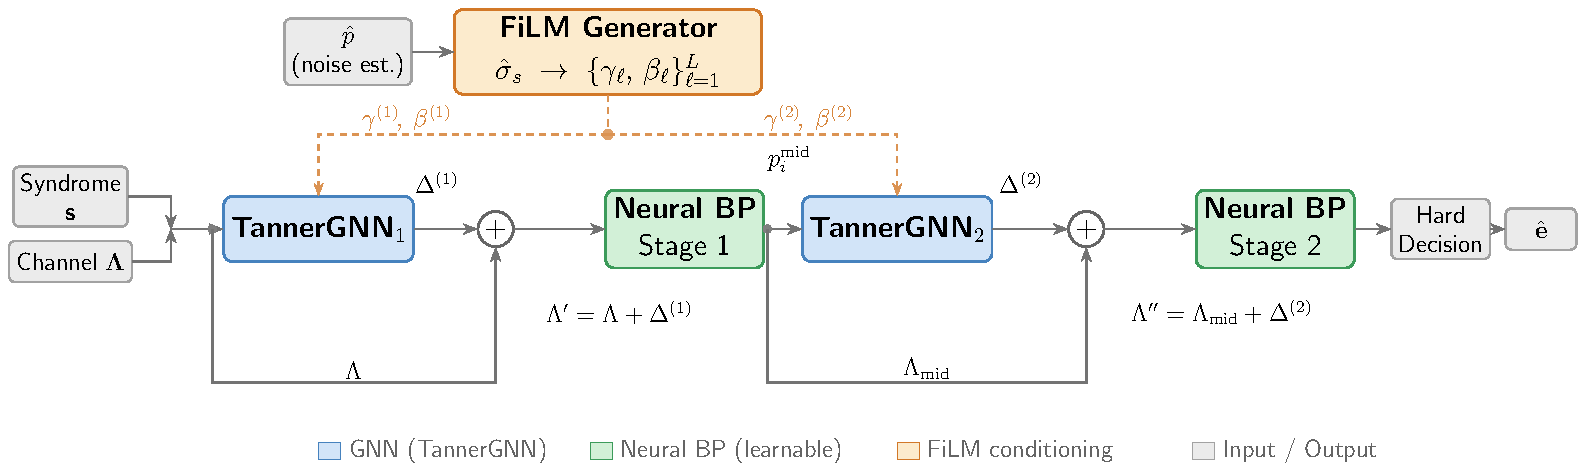
\includegraphics[width=\textwidth]{fig_interleaved_pipeline}
\caption{Interleaved GNN-BP pipeline. The GNN applies two successive
         LLR corrections: one before BP initialisation and one after
         $T_1$ iterations, using the mid-decoding posterior as an
         additional input. Both stages are trained end-to-end through
         the BP unroll.}
\label{fig:interleaved_pipeline}
\end{figure*}

\subsection{Training}\label{sec:training}

\begin{table}[t]
\centering
\caption{Configuration of the \textsc{TannerGNN} model behind
         Sec.~\ref{sec:gnn_positive} and Sec.~\ref{sec:mismatch}.}
\label{tab:hparams}
\resizebox{\columnwidth}{!}{%
\begin{tabular}{@{}ll@{}}
\toprule
\multicolumn{2}{@{}l}{\textit{Architecture}} \\
\midrule
Message-passing layers / hidden width & 3 / 32 \\
Node features                         & 4 (value, one-hot node type) \\
Residual connections, layer norm      & yes \\
FiLM / attention                      & not used \\
Parameters                            & 39{,}329 \\
\midrule
\multicolumn{2}{@{}l}{\textit{Training}} \\
\midrule
Data & 8{,}000 shots, sinusoidal drift, $p\in[0.005,0.045]$ \\
Loss & focal, $\alpha=0.25$, $\gamma=2$, on $\mathbf{e}_z$ \\
Optimiser & AdamW, lr $2\times10^{-3}$, weight decay $10^{-4}$ \\
Batch size / epochs & 64 / 20, gradient clipping 1.0 \\
Checkpoint & lowest failures on 4{,}000 validation shots \\
Training seeds & 5 \\
\midrule
\multicolumn{2}{@{}l}{\textit{Decoders}} \\
\midrule
BP (training and Table~\ref{tab:gnn_flooding}) & flooding min-sum, scaling 0.8, 10 iter. \\
BP-OSD reference & serial min-sum, scaling 0.8, 100 iter., OSD-CS-10 \\
\bottomrule
\end{tabular}}
\end{table}

\paragraph{Training loss.} For a shot with prior LLR
$\ell=\ln\bigl((1-p)/p\bigr)$ on every qubit, the GNN outputs a correction
$\delta_j$ for each qubit $j$, giving the corrected error probability
$q_j=\sigma\bigl(-(\ell+\delta_j)\bigr)$. The model is trained on the
focal loss~\cite{Lin2017Focal} against the true $Z$ error
$\mathbf{e}_z$,
\begin{equation}
\mathcal{L}=-\frac{1}{Bn}\sum_{b=1}^{B}\sum_{j=1}^{n}
\alpha_{t}\,(1-q_{t})^{\gamma}\log q_{t},
\label{eq:loss}
\end{equation}
where $q_t=q_j$ and $\alpha_t=\alpha$ if $e_{z,j}=1$, and
$q_t=1-q_j$ and $\alpha_t=1-\alpha$ otherwise, with $\alpha=0.25$ and $\gamma=2$. No syndrome-consistency term is used
for this model. At decoding time the corrected LLRs $\ell+\delta_j$ are
passed to both CSS components. The earlier FiLM and interleaved models
additionally used a syndrome-consistency term, the binary cross-entropy
between the measured syndrome and
$\tfrac12\bigl(1-\prod_{j\in\mathcal N(c)}(1-2q_j)\bigr)$ for each check
$c$ (weight $0.1$ in the configuration of the previous version).

The training data and splits of the headline experiment are described in
Sec.~\ref{sec:gnn_positive}; the configuration is summarised in
Table~\ref{tab:hparams}.

% ============================================================
%  IV. EXPERIMENTAL SETUP
% ============================================================
\section{Experimental Setup}\label{sec:setup}

\begin{figure*}[t]
\centering
\includegraphics[width=\textwidth]{fig_experimental_pipeline}
\caption{Experimental evaluation pipeline. Syndromes are sampled under
         static or drift noise models; each decoder receives identical
         syndrome batches to enable McNemar paired testing. Oracle
         experiments substitute true per-qubit rates for the uniform
         mean prior.}
\label{fig:experimental_pipeline}
\end{figure*}

\subsection{Evaluation regimes}\label{sec:regimes}

Two distinct evaluation regimes are used throughout this paper,
and the distinction is central to interpreting the results:

\textbf{Regime A (training-aligned baseline):} The GNN is evaluated
against flooding BP, the base decoder used during training. This
comparison isolates the gain relative to the decoder represented in the
training computation graph.

\textbf{Regime B (stronger classical baseline):} The same learned
correction is evaluated with the serial-schedule min-sum BP-OSD reference
configuration. This tests whether the correction also improves the
stronger classical decoder considered here; Sec.~\ref{sec:mismatch}
shows that it does not in the tested regime.

Unless otherwise stated, all experiments use $Z$-biased noise with
$\eta = 20$.

\subsection{Statistical protocol}\label{sec:metrics}

\paragraph{Logical failure.}
For each shot let $\hat{\mathbf{e}}_z$ and $\hat{\mathbf{e}}_x$ be the
decoder's hard decisions and let
$\mathbf{r}_z=\mathbf{e}_z\oplus\hat{\mathbf{e}}_z$ and
$\mathbf{r}_x=\mathbf{e}_x\oplus\hat{\mathbf{e}}_x$ be the residual
errors. A shot is counted as a logical failure if either
(i) the estimate does not reproduce the measured syndrome,
$\Hmat_x\hat{\mathbf{e}}_z\neq\mathbf{s}_x$ or
$\Hmat_z\hat{\mathbf{e}}_x\neq\mathbf{s}_z$; or
(ii) the syndrome is reproduced but the residual acts nontrivially on the
code space, $\mathbf{L}_x\mathbf{r}_z\neq\mathbf{0}$ or
$\mathbf{L}_z\mathbf{r}_x\neq\mathbf{0}$ over $\F_2$, where the rows of
$\mathbf{L}_x$ ($\mathbf{L}_z$) span the $k=12$ independent $X$-type
($Z$-type) logical operators modulo stabilizers. Condition (i) is required
because a syndrome-inconsistent residual is not a logical operator, so its
parity against a fixed set of logical representatives is not meaningful;
non-converged BP outputs are therefore always counted as failures. The
$X$- and $Z$-components are combined by logical OR, so the reported LER is
the probability that at least one of the 12 encoded qubits suffers a
logical error of any Pauli type in a single shot. At circuit level the same
rule is applied to the detector error model: a shot fails if the decoded
fault set does not reproduce the observed detection events, or if it does
and its predicted observable flips differ from the true ones.

For absolute LER comparisons we treat operating points with fewer than
100 observed logical-error events as preliminary; this is a reporting
heuristic rather than a formal power calculation. Decoder pairs are
evaluated on \emph{identical} syndrome samples, enabling paired
McNemar tests~\cite{McNemar1947}. We report Wilson score 95\% confidence
intervals for LER estimates.

Training, validation and test data are drawn with distinct random seeds,
so no evaluation shot shares a random stream with a training shot, and
learned-decoder results are reported over five training seeds
(initialisation and minibatch order). All training and evaluation used CPU
only; no GPU was available for this work. One training epoch of the
39k-parameter model of Sec.~\ref{sec:gnn_positive} takes about 16\,s on
four CPU cores.

% ============================================================
%  V. RESULTS
% ============================================================
\section{Results}\label{sec:results}

\subsection{Decoder configuration sensitivity}\label{sec:baseline}

Before presenting the GNN results, we quantify the sensitivity of the
classical baseline to decoder configuration. This sensitivity sets the
scale against which the learned-decoder results must be interpreted.

\begin{table*}[t]
\centering
\caption{Effect of BP-OSD configuration on $\code{288}{12}{18}$, $p=0.04$,
         $\eta=20$, $100{,}000$ identical shots, separate-CSS decoding with
         priors $p_Z=p\eta/(\eta+1)$, $p_X=p/(\eta+1)$. 95\% Wilson intervals
         in brackets. OSD is OSD-CS of order 10.}
\label{tab:smoking_gun}
\begin{tabular}{@{}llllcc@{}}
\toprule
Config & Schedule & Method & Iter & LER & Errors \\
\midrule
BP              & parallel & prod-sum & 30  & 0.0569 [0.0555, 0.0583] & 5{,}689 \\
BP              & serial   & ms(0.8)  & 100 & 0.00174 [0.00150, 0.00202] & 174 \\
BP-OSD          & parallel & prod-sum & 30  & 0.0398 [0.0386, 0.0411] & 3{,}983 \\
BP-OSD          & serial   & ms(0.8)  & 100 & 0.00034 [0.00024, 0.00048] & 34 \\
\bottomrule
\end{tabular}
\end{table*}

Table~\ref{tab:smoking_gun} illustrates how strongly decoder
configuration changes the finite-length result on $100{,}000$ identical
shots. Parallel product-sum BP-OSD with 30 iterations lowers the LER of the
corresponding plain BP only from $0.0569$ to $0.0398$, whereas serial
min-sum BP with 100 iterations reaches $0.0017$ without OSD and $0.00034$
with it, more than two orders of magnitude below the parallel
product-sum configurations.

A separate $100{,}000$-shot experiment (Fig.~\ref{fig:baseline_decomp})
changes one factor at a time. The flooding comparator is min-sum BP with
scaling factor $0.8$, at most 100 iterations, stopping at the first
iteration whose hard decision satisfies the syndrome, with a parallel
(flooding) schedule; the second decoder is identical except for the serial
schedule; the third adds OSD-CS-10. The logical error rate falls from
$1.28\times10^{-2}$ to $1.45\times10^{-3}$ ($8.8\times$, paired
$n_{10}/n_{01}=1138/3$) and then to $2.7\times10^{-4}$ ($5.4\times$,
$118/0$), about $47\times$ overall.

\begin{figure}[t]
\centering
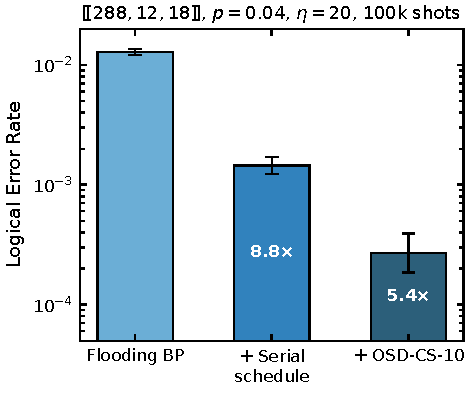
\includegraphics[width=\columnwidth]{fig_F1_baseline_decomp}
\caption{Baseline decomposition on $\code{288}{12}{18}$, $p=0.04$,
         $\eta=20$, 100k identical shots. Min-sum BP (scaling 0.8, at most
         100 iterations) with flooding and then serial schedule, then serial
         BP-OSD-CS-10. Bars: LER with 95\% Wilson intervals; labels give the
         factor gained at each step.}
\label{fig:baseline_decomp}
\end{figure}

These data do not identify a universally optimal configuration. They do
show that schedule, update rule, iteration budget, and post-processing
can dominate the measured finite-length LER. Learned-decoder comparisons
must therefore specify and control these parameters.

\subsection{Uniform-prior scaling invariance of min-sum BP}\label{sec:invariance}

\begin{proposition}[Uniform positive-scaling invariance]\label{prop:invariance}
Consider separate-CSS min-sum BP with no message clipping or offset. If
all channel LLRs in one CSS component are multiplied by the same factor
$a>0$, then every BP message and posterior LLR is multiplied by $a$ at
every iteration. Consequently, all hard decisions are unchanged.
\end{proposition}

\begin{proof}
At initialization, each variable-to-check message is proportional to the
corresponding channel LLR and therefore scales by $a$. Assume all
variable-to-check messages at iteration $t$ have scaled by $a$. The
syndrome factor $(-1)^{s_j}$ in Eq.~\eqref{eq:ctv} is unchanged, the sign
of every message is unchanged because $a>0$, and
$\min_i a|x_i|=a\min_i|x_i|$. Hence every check-to-variable message also
scales by $a$. Equation~\eqref{eq:vtc} then shows that the next
variable-to-check messages scale by $a$. Induction establishes the claim
for all iterations and for the final posterior LLRs.
\end{proof}

For a uniform channel prior, replacing a common positive LLR $\Lambda$
by another positive value $\Lambda'$ is equivalent to the scaling
$a=\Lambda'/\Lambda$. The proposition explains why changing only the assumed uniform physical
error rate cannot change hard decisions of ideal min-sum BP. Clipping, offsets, damping rules that depend on
magnitude, non-uniform priors, or sum-product updates can break the exact
scaling argument.

We checked the proposition on 2{,}000 shots each. With ldpc min-sum BP
(serial or flooding, 100 iterations), changing the assumed uniform rate
from $p=0.015$ to $0.0286$ on $\code{288}{12}{18}$, or from $0.04$ to
$0.02$ on $\code{72}{12}{6}$, leaves every hard decision unchanged
(2{,}000/2{,}000), and an assumed-bias sweep
$\eta\in\{1,2,5,10,20,50,100\}$ at $p=0.03$ gives identical decisions at
every value. Two cases fall outside the proposition, and the invariance
fails there: our PyTorch min-sum implementation clamps messages to
$\pm20$ and changes 18/2{,}000 decisions on $\code{288}{12}{18}$, and
sum-product BP changes 25--43 of 2{,}000.

\begin{remark}[What the proposition does and does not imply]
The result applies to the BP pathway when adaptivity enters only by
changing a uniform channel-prior magnitude. It does \emph{not} establish
that a global conditioning scalar is information-theoretically useless
to a GNN: a learned model could combine a global noise estimate with
local syndrome structure and change its nonlinear decision rule. The experiments below test a narrower hypothesis: spatially resolved
per-qubit calibration can change the relative reliabilities seen by the
decoder, whereas a single graph-wide scalar cannot provide that spatial
information.
\end{remark}

\subsection{GNN improvement over flooding BP}\label{sec:gnn_positive}

We evaluated the GNN against flooding BP, the decoder it was trained
against. The training set is 8{,}000 shots from two sinusoidally drifting
streams, $p(t)=p_0+0.015\sin(2\pi t/500)$ with $p_0\in\{0.02,0.03\}$, so
the training rates span $p\in[0.005,0.045]$. Validation (4{,}000 shots at
$p=0.04$) and test sets (20{,}000 shots at $p=0.04$, inside the training
range; 10{,}000 shots at $p=0.06$, outside it) are drawn with separate
random seeds. The checkpoint is chosen by the lowest validation failure
count over 20 epochs, each test set is scored once on that checkpoint, and
training is repeated with five seeds (Table~\ref{tab:hparams}).

\begin{table}[t]
\centering
\caption{GNN-BP vs.\ flooding BP on $\code{72}{12}{6}$, $\eta=20$, five training seeds (mean $\pm$ s.d.).
Failures follow the definition in Sec.~\ref{sec:metrics}.
95\% Wilson intervals for single decoders are $\pm0.004$ at $p=0.04$
and $\pm0.009$ at $p=0.06$.}
\label{tab:gnn_flooding}
\resizebox{\columnwidth}{!}{%
\begin{tabular}{@{}lcc@{}}
\toprule
Decoder & $p=0.04$ ($20$k shots) & $p=0.06$ ($10$k shots)\\
\midrule
BP, 10 iter. & 0.1077 & 0.2867\\
GNN + BP, 10 iter. & $0.0942\pm0.0006$ & $0.2564\pm0.0019$\\
\quad relative reduction & $12.5\%\pm0.6\%$ & $10.6\%\pm0.7\%$\\
\quad McNemar $n_{10}/n_{01}$ (range) & 313--370 / 64--95 & 343--394 / 66--80\\
BP, 100 iter. & 0.0863 & 0.2403\\
Serial BP-OSD-CS(10), 100 iter. & 0.0707 & 0.2138\\
\bottomrule
\end{tabular}}
\end{table}

GNN pre-processing reduces the failure rate of 10-iteration BP by
$12.5\%\pm0.6\%$ at $p=0.04$ and $10.6\%\pm0.7\%$ at $p=0.06$, which lies
outside the training range; every seed is significant
($p<10^{-36}$, McNemar). The gain comes mostly from convergence: shots where
BP fails to reproduce the syndrome fall from 1{,}740 to 838--975 of 20{,}000.
The gain does not close the gap to longer decoding: 100-iteration BP (0.0863)
and serial BP-OSD (0.0707) both outperform GNN + 10-iteration BP.

On the original single-seed checkpoint, a gradient audit found non-zero
signal through the network (input-to-readout gradient ratio $0.22$) and
non-trivial LLR corrections (mean $|\Delta_i|=0.854$).

A fixed-dataset capacity test provides an additional diagnostic: a GNN
trained on 1{,}000 fixed syndromes for 50 epochs reduced the failure count
on those same syndromes from 105 to 93 ($11\%$; $n_{10}=15$, $n_{01}=3$,
McNemar $p=0.0095$). This experiment tests the ability of the architecture and
optimizer to fit the supplied examples; it is not a generalization
result. The interleaved architecture of Sec.~\ref{sec:neuralbp} is not evaluated in this work.


\subsection{Training/evaluation baseline mismatch}\label{sec:mismatch}

Although the GNN improves flooding BP, the same correction does not
improve the serial min-sum BP-OSD reference configuration. We pass the
corrected LLRs of each of the five trained models to BP-OSD and compare
with BP-OSD alone on 20{,}000 identical fresh shots per error rate
(Table~\ref{tab:gnn_null}); these shots differ from the test sets of
Table~\ref{tab:gnn_flooding}.

\begin{table}[t]
\centering
\caption{GNN+OSD vs.\ serial BP-OSD on $\code{72}{12}{6}$, $\eta=20$,
         $20{,}000$ identical shots per $p$, five GNN training seeds.
         Serial min-sum BP-OSD-CS-10 (scaling 0.8, 100 iterations).}
\label{tab:gnn_null}
\resizebox{\columnwidth}{!}{%
\begin{tabular}{@{}lccc@{}}
\toprule
$p$ & Serial BP-OSD & GNN+OSD (5 seeds) & Seeds worse ($p_\mathrm{McN}<0.05$) \\
\midrule
0.02 & 0.0093 & 0.0095--0.0102 & 1/5 \\
0.03 & 0.0297 & 0.0306--0.0317 & 5/5 \\
0.04 & 0.0676 & 0.0688--0.0709 & 4/5 \\
0.05 & 0.1354 & 0.1384--0.1418 & 5/5 \\
\bottomrule
\end{tabular}}
\end{table}

\begin{figure}[t]
\centering
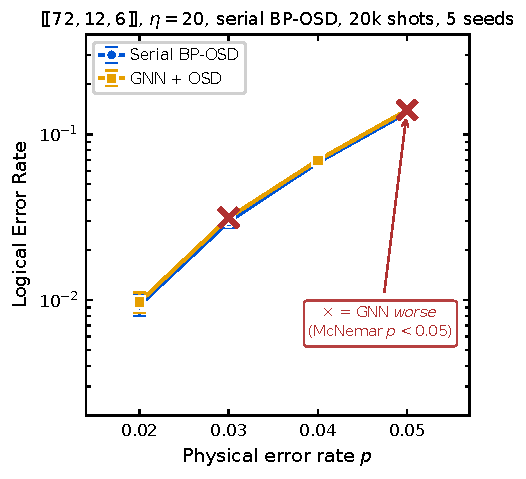
\includegraphics[width=\columnwidth]{fig_F4_phase4_ler}
\caption{GNN+OSD vs.\ serial BP-OSD LER on $\code{72}{12}{6}$,
         $\eta=20$, 20{,}000 shots per point; GNN+OSD is the mean over
         five training seeds. Red $\times$ marks operating points where
         every seed is statistically worse (McNemar $p<0.05$).
         Wilson 95\% CI error bars.}
\label{fig:gnn_null_curve}
\end{figure}

Table~\ref{tab:gnn_null} and Fig.~\ref{fig:gnn_null_curve} show that the
GNN-corrected decoder never improves on serial BP-OSD: at $p=0.02$ only one
seed of five is significantly worse, and from $p=0.03$ on 14 of 15
seed--error-rate pairs are significantly \emph{worse}. The same checkpoints
improve flooding BP, so the learned correction does not transfer unchanged
to the stronger decoder.

\begin{table}[t]
\centering
\caption{Paired failure sets on $\code{72}{12}{6}$, $p=0.04$, $\eta=20$,
         $20{,}000$ identical held-out shots. BP: 10-iteration flooding
         min-sum (the GNN's training decoder). GNN rows give the range over
         five training seeds. ``Non-conv.'': the estimate does not reproduce
         the syndrome.}
\label{tab:failure_sets}
\resizebox{\columnwidth}{!}{%
\begin{tabular}{@{}lcc@{}}
\toprule
Decoder & Failures & Non-conv. \\
\midrule
BP, 10 iter.            & 2{,}155 & 1{,}740 \\
BP, 100 iter.           & 1{,}727 & 700 \\
Serial BP-OSD           & 1{,}414 & 0 \\
GNN + BP, 10 iter.      & 1{,}874--1{,}906 & 838--975 \\
GNN + BP-OSD            & 1{,}439--1{,}451 & 0 \\
\midrule
\multicolumn{3}{@{}l}{\textit{Overlaps}} \\
BP-OSD failures that BP also fails & \multicolumn{2}{c}{1{,}319 / 1{,}414 (93\%)} \\
BP-100 failures that BP also fails & \multicolumn{2}{c}{1{,}727 / 1{,}727 (100\%)} \\
Shots GNN fixes for BP (BP fails, GNN+BP succeeds) & \multicolumn{2}{c}{313--370} \\
\quad of which BP did not converge & \multicolumn{2}{c}{91--93\%} \\
\quad of which BP-OSD also fails & \multicolumn{2}{c}{31--36\%} \\
BP-OSD failures that GNN+BP also fails & \multicolumn{2}{c}{87--88\%} \\
GNN+BP-OSD vs.\ BP-OSD: newly failed / rescued & \multicolumn{2}{c}{237--282 / 206--254} \\
\quad newly failed shots that BP also fails & \multicolumn{2}{c}{91--95\%} \\
\bottomrule
\end{tabular}}
\end{table}

Table~\ref{tab:failure_sets} compares the failure sets of all decoders on
identical shots. The failure sets are nested rather than disjoint: every
shot that 100-iteration BP fails is also failed by 10-iteration BP, and
93\% of BP-OSD's failures are BP failures. What separates the decoders is
mainly convergence: 81\% of 10-iteration BP failures are shots on which BP
does not reach a syndrome-consistent estimate, whereas BP-OSD always
returns one. No decoder fails on any error of weight $\le 2=(d-1)/2$;
all failures involve errors of weight at least 3 (mean weight 5.4--5.7).
In 1{,}411 of BP-OSD's 1{,}414 failures the returned correction is
syndrome-consistent and no heavier than the true error, so these failures
are limited by the code and the noise, not by a decoder returning an
unnecessarily heavy estimate.

The GNN's gains lie where BP-OSD already succeeds. Of the 313--370 shots
the GNN fixes for 10-iteration BP, 91--93\% are shots on which BP did not
converge, and only 31--36\% are shots that BP-OSD fails; conversely,
GNN+BP still fails 87--88\% of BP-OSD's failures. When the same
corrections are passed to BP-OSD, they reshuffle rather than remove its
failures (237--282 newly failed vs.\ 206--254 rescued shots), almost
entirely among the hard shots on which BP itself fails. They also make
OSD return heavier incorrect estimates (20--43 failures with an estimate
heavier than the true error, vs.\ 3 for BP-OSD alone). The same pattern
holds at $p=0.06$ (10{,}000 shots): 96\% of BP-OSD failures are BP
failures, and 30--36\% of the GNN's fixes are BP-OSD failures.

The GNN was optimized through a 10-iteration flooding-BP computation graph
and is then inserted ahead of a decoder with a different schedule,
iteration budget, and OSD post-processing. Training directly against the
target decoder, or against a differentiable surrogate of its
post-processing stage, remains the appropriate test of whether learned
augmentation can improve BP-OSD.

\subsection{Per-qubit calibration gap}\label{sec:oraclegap}

Under spatially non-uniform per-qubit noise, each data qubit has rate
$p_i=p\,e^{\sigma z_i-\sigma^2/2}$ with $z_i\sim\mathcal N(0,1)$ drawn
fresh every shot (capped at 0.5), so the mean rate is $p$ for every
$\sigma$; the mean-prior decoder uses the uniform rate $p$. A decoder knowing the true per-qubit rates
(serial min-sum BP-OSD-CS-10 with the true $p_i$ as priors) substantially
outperforms the mean-prior decoder.

\begin{figure}[t]
\centering
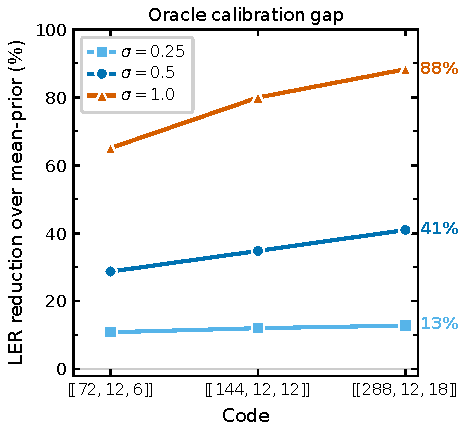
\includegraphics[width=\columnwidth]{fig_F2_oracle_vs_distance}
\caption{Oracle calibration gap (percentage LER reduction of
         per-qubit-oracle over mean-prior BP-OSD), 50k identical shots per
         point. Operating points: $p=0.04$, $0.06$, $0.07$ for the three
         codes; cross-code comparisons are partially confounded by the
         differing operating points.}
\label{fig:oracle_gap}
\end{figure}

\begin{table*}[t]
\centering
\caption{Oracle gap: percentage LER reduction of per-qubit-oracle over
         mean-prior serial BP-OSD-CS-10, $50{,}000$ identical shots per
         cell. Parentheses: mean-prior failures. McNemar
         $p<10^{-20}$ in the upper three rows and $p<10^{-5}$ in the last.
         The upper three rows use the operating points of
         Fig.~\ref{fig:oracle_gap}; the last row fixes $p=0.04$.}
\label{tab:oracle}
\begin{tabular}{@{}llccc@{}}
\toprule
Code ($d$) & $p$ & $\sigma=0.25$ & $\sigma=0.5$ & $\sigma=1.0$ \\
\midrule
$\code{72}{12}{6}$   (6)  & 0.04 & $10.8\%$ (3508) & $28.7\%$ (3432) & $65.1\%$ (3438) \\
$\code{144}{12}{12}$ (12) & 0.06 & $12.0\%$ (3165) & $34.8\%$ (3203) & $79.9\%$ (2936) \\
$\code{288}{12}{18}$ (18) & 0.07 & $12.8\%$ (3338) & $40.9\%$ (3307) & $88.3\%$ (2786) \\
\midrule
$\code{144}{12}{12}$ (12) & 0.04 & $19.8\%$ (324)  & $45.5\%$ (275)  & $85.3\%$ (278) \\
\bottomrule
\end{tabular}
\end{table*}

Table~\ref{tab:oracle} and Fig.~\ref{fig:oracle_gap} show a clear
increase with noise contrast $\sigma$ for each tested code. The reported
percentage reduction is also larger for the larger-code rows, reaching
$88\%$ on $\code{288}{12}{18}$ at $\sigma=1.0$; however, the physical
error rate is changed across codes ($p=0.04$, $0.06$, and $0.07$).
At a common $p=0.04$, $\code{144}{12}{12}$ shows larger gaps than
$\code{72}{12}{6}$ at every $\sigma$ (Table~\ref{tab:oracle}, last row),
but $\code{288}{12}{18}$ fails too rarely at that rate to resolve the
trend. These data therefore do not isolate code distance as the cause of
the cross-code trend.

This experiment isolates the value of synthetic per-qubit rate side
information; it does not require machine learning. We use the true-rate
decoder as an \emph{oracle reference}, not as a formal upper bound on all
possible decoders. The comparison quantifies how much the tested BP-OSD
implementation can benefit when the realized per-qubit rates are
revealed. The gap is \emph{not}
recoverable from a single syndrome shot under i.i.d.\ per-qubit
noise: with a fresh field redrawn every shot, the uniform mean
prior is Bayes-optimal within the class of estimators that observe
only the syndrome, so no syndrome-conditioned GNN can do better
than the mean prior in this regime.

\subsection{Circuit-level evaluation}\label{sec:circuit}

\paragraph{Circuit and noise model.}
We simulate a $Z$-basis memory experiment on $\code{72}{12}{6}$ with
6 rounds of syndrome extraction. Data qubits are prepared in $\ket{0}$;
each round measures all 36 $X$-checks and then all 36 $Z$-checks with
dedicated ancillas, using CNOT layers from a greedy conflict-free schedule;
the data qubits are finally measured in the $Z$ basis. Detectors are
(i) the 36 $Z$-checks of round 1, which are deterministic for the prepared
state, (ii) the XOR of consecutive measurements of every check in rounds
2--6, and (iii) the XOR of the last $Z$-check outcome with the parity of the
measured data qubits in its support, giving 432 detectors and 12 logical
observables (the $Z$-type logical operators). Noise is a biased single-qubit
Pauli channel with $p_X=p/(\eta+1)$, $p_Z=p\,\eta/(\eta+1)$, $p_Y=0$,
$\eta=20$, applied to every qubit after each one- and two-qubit gate and to
every idle qubit at each time step; measurements and resets flip with
probability $p$. Under spatially non-uniform noise each qubit $q$ (data and
ancilla) has rate $p_q=p_\mathrm{mean}e^{\sigma z_q}$, $z_q\sim\mathcal N(0,1)$,
$\sigma=1$, on all of its fault locations.

\paragraph{Decoders.}
We decode the detector error model (DEM; 4{,}068 fault mechanisms) with
BP-OSD (min-sum, scaling $0.625$, serial schedule, 100 iterations, OSD-CS
order 10). The \emph{mean-prior} decoder uses a uniform rate equal to the
log-normal mean $p_\mathrm{mean}e^{\sigma^2/2}$; the \emph{oracle} uses the
true $p_q$. We draw 20 (40) rate profiles at $p_\mathrm{mean}\le0.003$
($0.006$) and 500 shots per profile. A shot fails if the decoded fault set
does not reproduce the detection events or predicts the wrong observable flips.

\begin{table}[t]
\centering
\caption{Circuit-level oracle gap on $\code{72}{12}{6}$ (6 rounds, $\eta=20$,
log-normal $\sigma=1$). $n_{10}$: shots only the mean-prior decoder fails;
$n_{01}$: shots only the oracle fails. The last column counts rate profiles
on which the mean-prior decoder has more failures than the oracle / fewer.}
\label{tab:circuit}
\resizebox{\columnwidth}{!}{%
\begin{tabular}{@{}lccccc@{}}
\toprule
$p_\mathrm{mean}$ & Shots & Mean-prior LER & Oracle LER & $n_{10}/n_{01}$ (McNemar $p$) & Profiles \\
\midrule
0.001 & 10{,}000 & $0$ ($<\!3.8\times10^{-4}$) & $0$ ($<\!3.8\times10^{-4}$) & 0/0 & 0/0 \\
0.003 & 10{,}000 & $1.4\times10^{-3}$ & $0.6\times10^{-3}$ & 9/1 (0.027) & 6/0 \\
0.006 & 20{,}000 & $1.36\times10^{-2}$ & $0.60\times10^{-2}$ & 192/39 ($1.5\times10^{-23}$) & 38/2 \\
\bottomrule
\end{tabular}}
\end{table}

\begin{figure}[t]
\centering
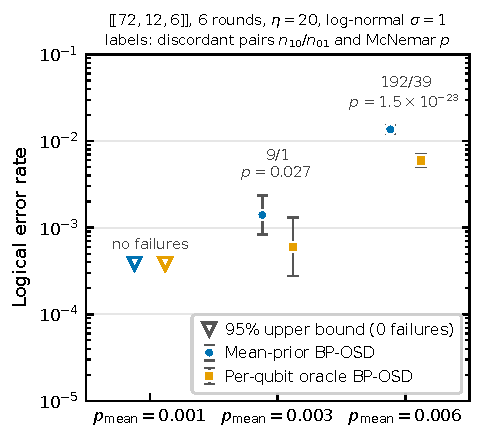
\includegraphics[width=\columnwidth]{fig_F6_circuit_oracle}
\caption{Circuit-level oracle gap on $\code{72}{12}{6}$. Points: logical
error rate with 95\% Wilson intervals; open triangles: 95\% upper bound when
no failures were observed. The per-qubit oracle has $56\%$ fewer failures
than the mean-prior decoder at $p_\mathrm{mean}=0.006$.}
\label{fig:circuit_oracle}
\end{figure}

Knowing the per-qubit rates also helps at circuit level
(Table~\ref{tab:circuit}, Fig.~\ref{fig:circuit_oracle}). At
$p_\mathrm{mean}=0.006$ the oracle reduces the logical error rate from
$1.36\%$ to $0.60\%$ ($56\%$; McNemar $p=1.5\times10^{-23}$), and it is
better on 38 of 40 independent rate profiles (sign test $p=1.5\times10^{-9}$),
so the result is not driven by a few extreme profiles. At
$p_\mathrm{mean}=0.003$ the gap has the same size ($57\%$) but only 10
discordant shots, and at $p_\mathrm{mean}=0.001$ neither decoder fails in
$10^4$ shots. The circuit-level gap ($56\%$) is somewhat smaller than the
code-capacity gap on the same code ($65.1\%$), but it does not vanish.

\paragraph{Correction to an earlier version.}
An earlier version of this section reported logical error rates of $0.27$ and
$0.34$ at $p_\mathrm{mean}=0.001$ and $0.003$ and no oracle gap. Those
circuits lacked the first-round and final detectors (360 instead of 432),
so any fault that flipped a logical near the time boundaries was invisible
to the decoder. This produced a logical error floor that no prior could
remove. With the complete detector set, uniform noise at $p=0.001$, $0.003$,
$0.005$ and $0.01$ gives $0/10^4$, $5/10^4$, $14/10^4$ and
$2.1\times10^{-2}$; the legacy circuit gives $0.124$ and $0.336$ at
$p=0.001$ and $0.003$.

% ============================================================
%  VI. DISCUSSION
% ============================================================
\section{Discussion}\label{sec:discussion}

\subsection{The GNN's role and its limits}

\textsc{TannerGNN} reduces the LER of the 10-iteration flooding BP
decoder used in its training loop by $12.5\%\pm0.6\%$ over five training
seeds, and the gain persists outside the training range. The mechanism is
mainly convergence: the GNN roughly halves the number of shots on which BP
fails to reach a syndrome-consistent estimate (1{,}740 to 838--975 of
20{,}000). Running BP for 100 iterations achieves more than this, and
BP-OSD more still, so the result is best read as a cheaper route to part
of the benefit of longer decoding, not as an improvement on
state-of-the-art BB decoding.

The Regime-B result follows from the failure-set structure
(Table~\ref{tab:failure_sets}): BP-OSD's failures are a near-subset of
BP's, and the GNN's repairs fall mostly on shots BP-OSD already decodes.
When passed to BP-OSD, the learned corrections reshuffle failures among
the hardest shots and make OSD choose heavier incorrect estimates, giving
a small net loss. Training against the target decoder, for example
through a differentiable surrogate of OSD or on the residual failures of
BP-OSD, is the appropriate next test.

\subsection{Benchmark design implications}

The baseline experiments identify two reporting requirements for learned
QLDPC decoders. First, BP-OSD schedule, update rule, iteration count, and
OSD configuration must be stated explicitly because they can change LER
by more than two orders of magnitude on the same code. Table~\ref{tab:hparams}
records these settings for the present study.

Second, the training and evaluation decoders must be distinguished. An
LLR correction learned through flooding BP need not remain beneficial
when the schedule, iteration count, and OSD stage are changed. Comparisons
across such decoder configurations should identify the mismatch rather
than treating all BP-based baselines as equivalent.

\subsection{Comparison with prior work}\label{sec:priorwork}

Astra~\cite{Maan2025MLBP} uses a learned Tanner-graph message-passing
decoder and reports BB-code performance competitive with, and in several
settings better than, BP-OSD under code-capacity depolarizing noise. This
places our $12.5\%$ flooding-BP gain in context: improvement over plain BP
is not, by itself, the main novelty. Our contribution is instead the
controlled comparison showing how that gain changes when the baseline
and side information are strengthened.

Gong et al.~\cite{Gong2024GNN} interleave differentiable BP stages with
GNN corrections on the same sparse graph and show error-floor
improvements over several post-processing approaches. Our interleaved
variant follows the same broad design principle, but its decoding
performance is not evaluated here, so we make no claim for that
architecture.

Recent circuit-level work on BB codes also reports neural decoders that
can outperform BP-OSD on the $\code{72}{12}{6}$ code while retaining a
runtime advantage, although scaling to $\code{144}{12}{12}$ remains more
challenging~\cite{Blue2026MLBB}. This comparison reinforces the need to evaluate learned decoders against
a fully specified competitive non-learned baseline, not only against
flooding BP.

Stein et al.~\cite{Stein2026FiLM} condition a neural QEC decoder on
spatially resolved hardware calibration data using FiLM and evaluate on
IBM repetition-code experiments. Their conditioning signal is per-qubit
and calibration-derived, unlike the single scalar $\phat$ used in our
initial model. This distinction is consistent with the oracle experiments
of Sec.~\ref{sec:oraclegap}, which motivate spatial rather than purely
global conditioning.
\subsection{Towards spatially-resolved conditioning}\label{sec:srcf}

The oracle-gap experiment (Sec.~\ref{sec:oraclegap}) shows that
per-qubit rate side information can materially improve the tested
BP-OSD decoder. Because operating point and code size co-vary, the
current data do not establish how this value scales with distance.
Proposition~\ref{prop:invariance} also shows that a uniform rescaling
of the min-sum BP prior cannot reproduce the effect of spatially varying
reliabilities. These results motivate testing spatially resolved FiLM
(SRCF), in which per-qubit parameters $(\gamma_i, \beta_i)$ are
conditioned on persistent hardware calibration data rather than on a
single graph-wide scalar. Such a decoder should be compared with a non-learned per-qubit frequency
estimator and evaluated at circuit level, where the oracle gap remains
large ($56\%$ at $p_\mathrm{mean}=0.006$, Sec.~\ref{sec:circuit}).
Whether such rates can be estimated well enough from syndrome history has
not been established in the present experiments.

\subsection{Limitations}\label{sec:limitations}

\begin{enumerate}[leftmargin=*,topsep=3pt,itemsep=2pt,label=(\roman*)]
\item The GNN was trained only through 10-iteration flooding BP. Training
      against serial BP-OSD, the competitive classical baseline, is untested.
\item GNN checkpoints exist only for $\code{72}{12}{6}$; the larger codes
      were not trained because of CPU-only compute. The Regime-B result
      should not be extrapolated to them.
\item The single per-qubit correction $\delta_j$ is trained on $Z$ errors
      and applied to both CSS components, which is suboptimal under
      $\eta=20$ biased noise; separate $Z$ and $X$ readout heads are the
      natural fix.
\item The interleaved architecture and the FiLM variant are described but
      their decoding performance is not evaluated.
\item The circuit-level study uses one code, 6 rounds and a biased
      single-qubit channel after each gate; two-qubit correlated faults,
      leakage and crosstalk are not modelled, and the paper's operating
      points $p_\mathrm{mean}\le0.003$ are too clean to resolve the gap.
\item Hyperparameter search and training duration were limited by CPU-only
      compute.
\end{enumerate}

% ============================================================
%  VII. CONCLUSION
% ============================================================
\section{Conclusion}\label{sec:conclusion}

On $\code{72}{12}{6}$, a Tanner-graph GNN trained through 10-iteration
flooding BP reduces that decoder's LER by $12.5\%\pm0.6\%$ at $p=0.04$
and $10.6\%\pm0.7\%$ at $p=0.06$, reproducibly over five training seeds
and on leakage-free held-out data. The gain comes mostly from helping BP
converge. It does not reach 100-iteration BP or serial BP-OSD, and the
same corrections make BP-OSD slightly worse because the shots they repair
are largely ones BP-OSD already decodes. An improvement over one BP
baseline therefore does not establish an improvement over a stronger
decoder.

Decoder configuration matters as much as the learned component: on
$\code{288}{12}{18}$, schedule and OSD post-processing alone change LER by
about $47\times$. We proved that uniform positive rescaling of the channel
LLRs leaves the hard decisions of unclipped min-sum BP unchanged, so a
global noise estimate cannot by itself make min-sum BP adaptive. Per-qubit
calibration, however, is highly informative: revealing true per-qubit
rates reduces BP-OSD's LER by up to $88\%$ at code capacity and by $56\%$
under circuit-level noise. The direct next test is a learned decoder
conditioned on persistent spatial calibration data, compared against a
fully specified serial BP-OSD baseline and a non-learned per-qubit
estimator.

\section*{Acknowledgments}

The authors thank the STAR Lab program at the University of Arizona
for facilitating this research and providing computational resources.

\section*{Data and code availability}

Source code, trained checkpoints, datasets and analysis scripts are
available at \url{https://github.com/kondshk/adaptive_gnn}.
All tables and figures are produced by a committed script from stored
per-shot outcomes: \texttt{audit\_headline\_v2.py} (headline result),
\texttt{audit\_tables\_v2.py} (baseline, invariance, BP-OSD and oracle
tables), \texttt{audit\_failure\_sets.py} (failure sets) and
\texttt{audit\_circuit\_v2.py} (circuit level); \texttt{docs/PROVENANCE.md}
maps each reported number to its source. Code-capacity data are sampled directly with NumPy;
circuit-level data are generated with Stim~\cite{Gidney2021Stim}.

\bibliographystyle{quantum}
\bibliography{references}

\end{document}
